\setcounter{figure}{0}
\setcounter{table}{0}
\section{测试与结论}
本章主要介绍对R峰检测算法与应用的测试,并且根据结果给出结论。

\subsection{R峰峰值检测算法的测试与结果}
选取PhysioNet提供的MIT-BIH心律失常库进行测试\cite{goldberger_physiobank_2000}\cite{moody_impact_2001}。该ECG数据库提供了真实收集的ECG数据,并且提供了心率数据以供参考。通过对10条持续时间为1min的ECG记录进行分析,得出的结果见下表。

\begin{table}[htbp]
  \centering
  \caption{R峰检测算法的测试结果 % 表头
  \label{t2}}
  \wuhao
\begin{tabular}{|c|c|c|c|c|c|c|c|c|c|c|c|}
\hline 
数据 & 100 & 101 & 103 & 105 & 106 & 114 & 115 & 116 & 118 & 122 & 总计 \\ 
\hline 
TP & 74 & 71 & 70 & 82 & 66 & 54 & 63 & 79 & 71 & 87 & 717 \\ 
\hline 
FN & 0 & 0 & 0 & 1 & 0 & 0 & 0 & 0 & 1 & 0 & 2 \\ 
\hline 
Se(\%) & 100 & 100 & 100 & 98.8 & 100 & 100 & 100 & 100 & 98.6 & 100 & 99.7 \\ 
\hline 
Ac(\%) & 100 & 100 & 100 & 98.8 & 100 & 100 & 100 & 100 & 98.6 & 100 & 99.7 \\ 
\hline 
\end{tabular}  
\end{table}

其中TP、FN均为病理统计中的方法,Se指敏感度,Ac指准确度\cite{department_of_statistics_online_programs_sensitivity_????}。表中TP指正确识别的R峰数量,FN指未识别出的R峰数量。由数据可看出R峰检测算法识别准确稳定,能够达到医疗应用的要求。

\subsection{ECG监测与记录应用的运行测试}
分别在LG G3(D857)和小米2S两种Android设备上安装ECG监测与记录应用,测试应用的各项功能。蓝牙发送功能由PC模拟。编写Python程序使用串口发送一段ECG信号记录,两种机型均能正常接收,且能正常识别R峰的出现。使用“导出数据”功能能够正常生成含有ECG记录的txt文本文件,说明数据库功能也运行正常。

应用识别一个周期内R峰出现、计算RR间期及心率的过程如图\ref{fig5-1}所示。可以看到,在探测到R峰后,应用显示出了即时的心率值和RR间期。同时用户可在屏幕上触摸以获取准确的R峰峰值。

\begin{figure}[htb]
  \centering
  \subfigure[探测到R峰前]{
    \label{fig5-1a} %% label for first subfigure
    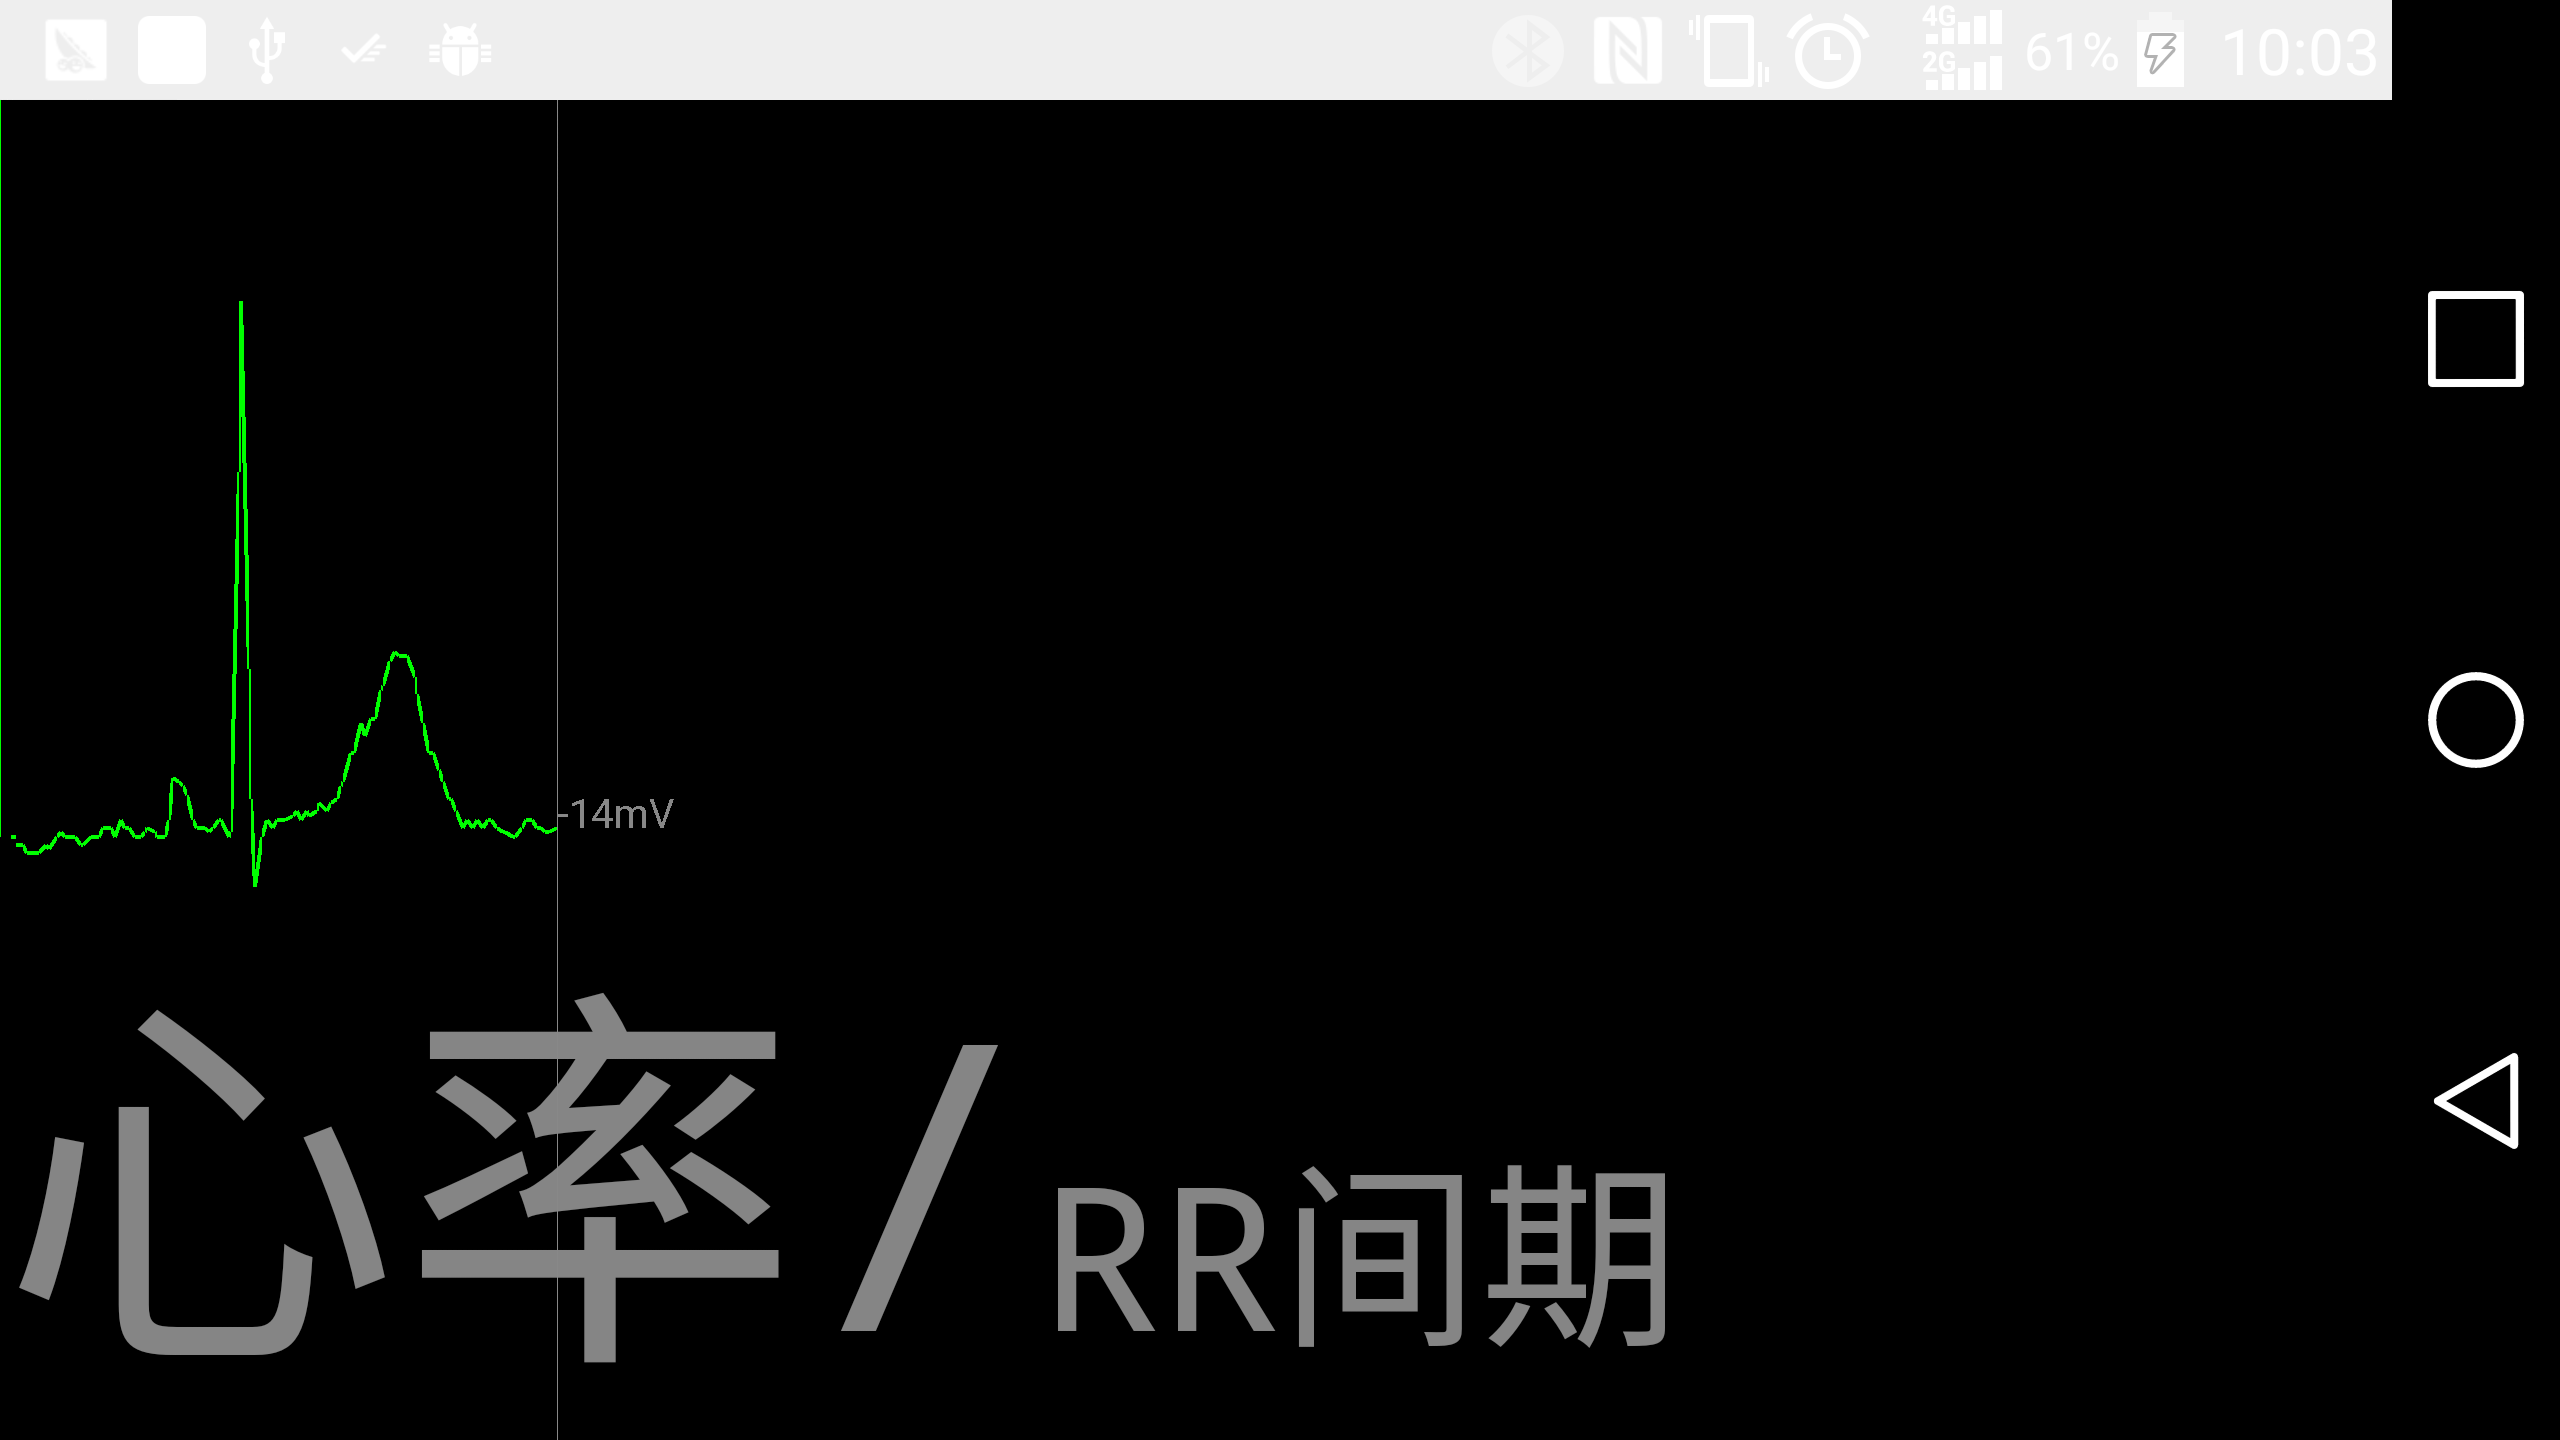
\includegraphics[width=0.6\textwidth]{fig5-1a.png}}
  \\
  \subfigure[探测到R峰并测量]{
    \label{fig5-1b} %% label for second subfigure
    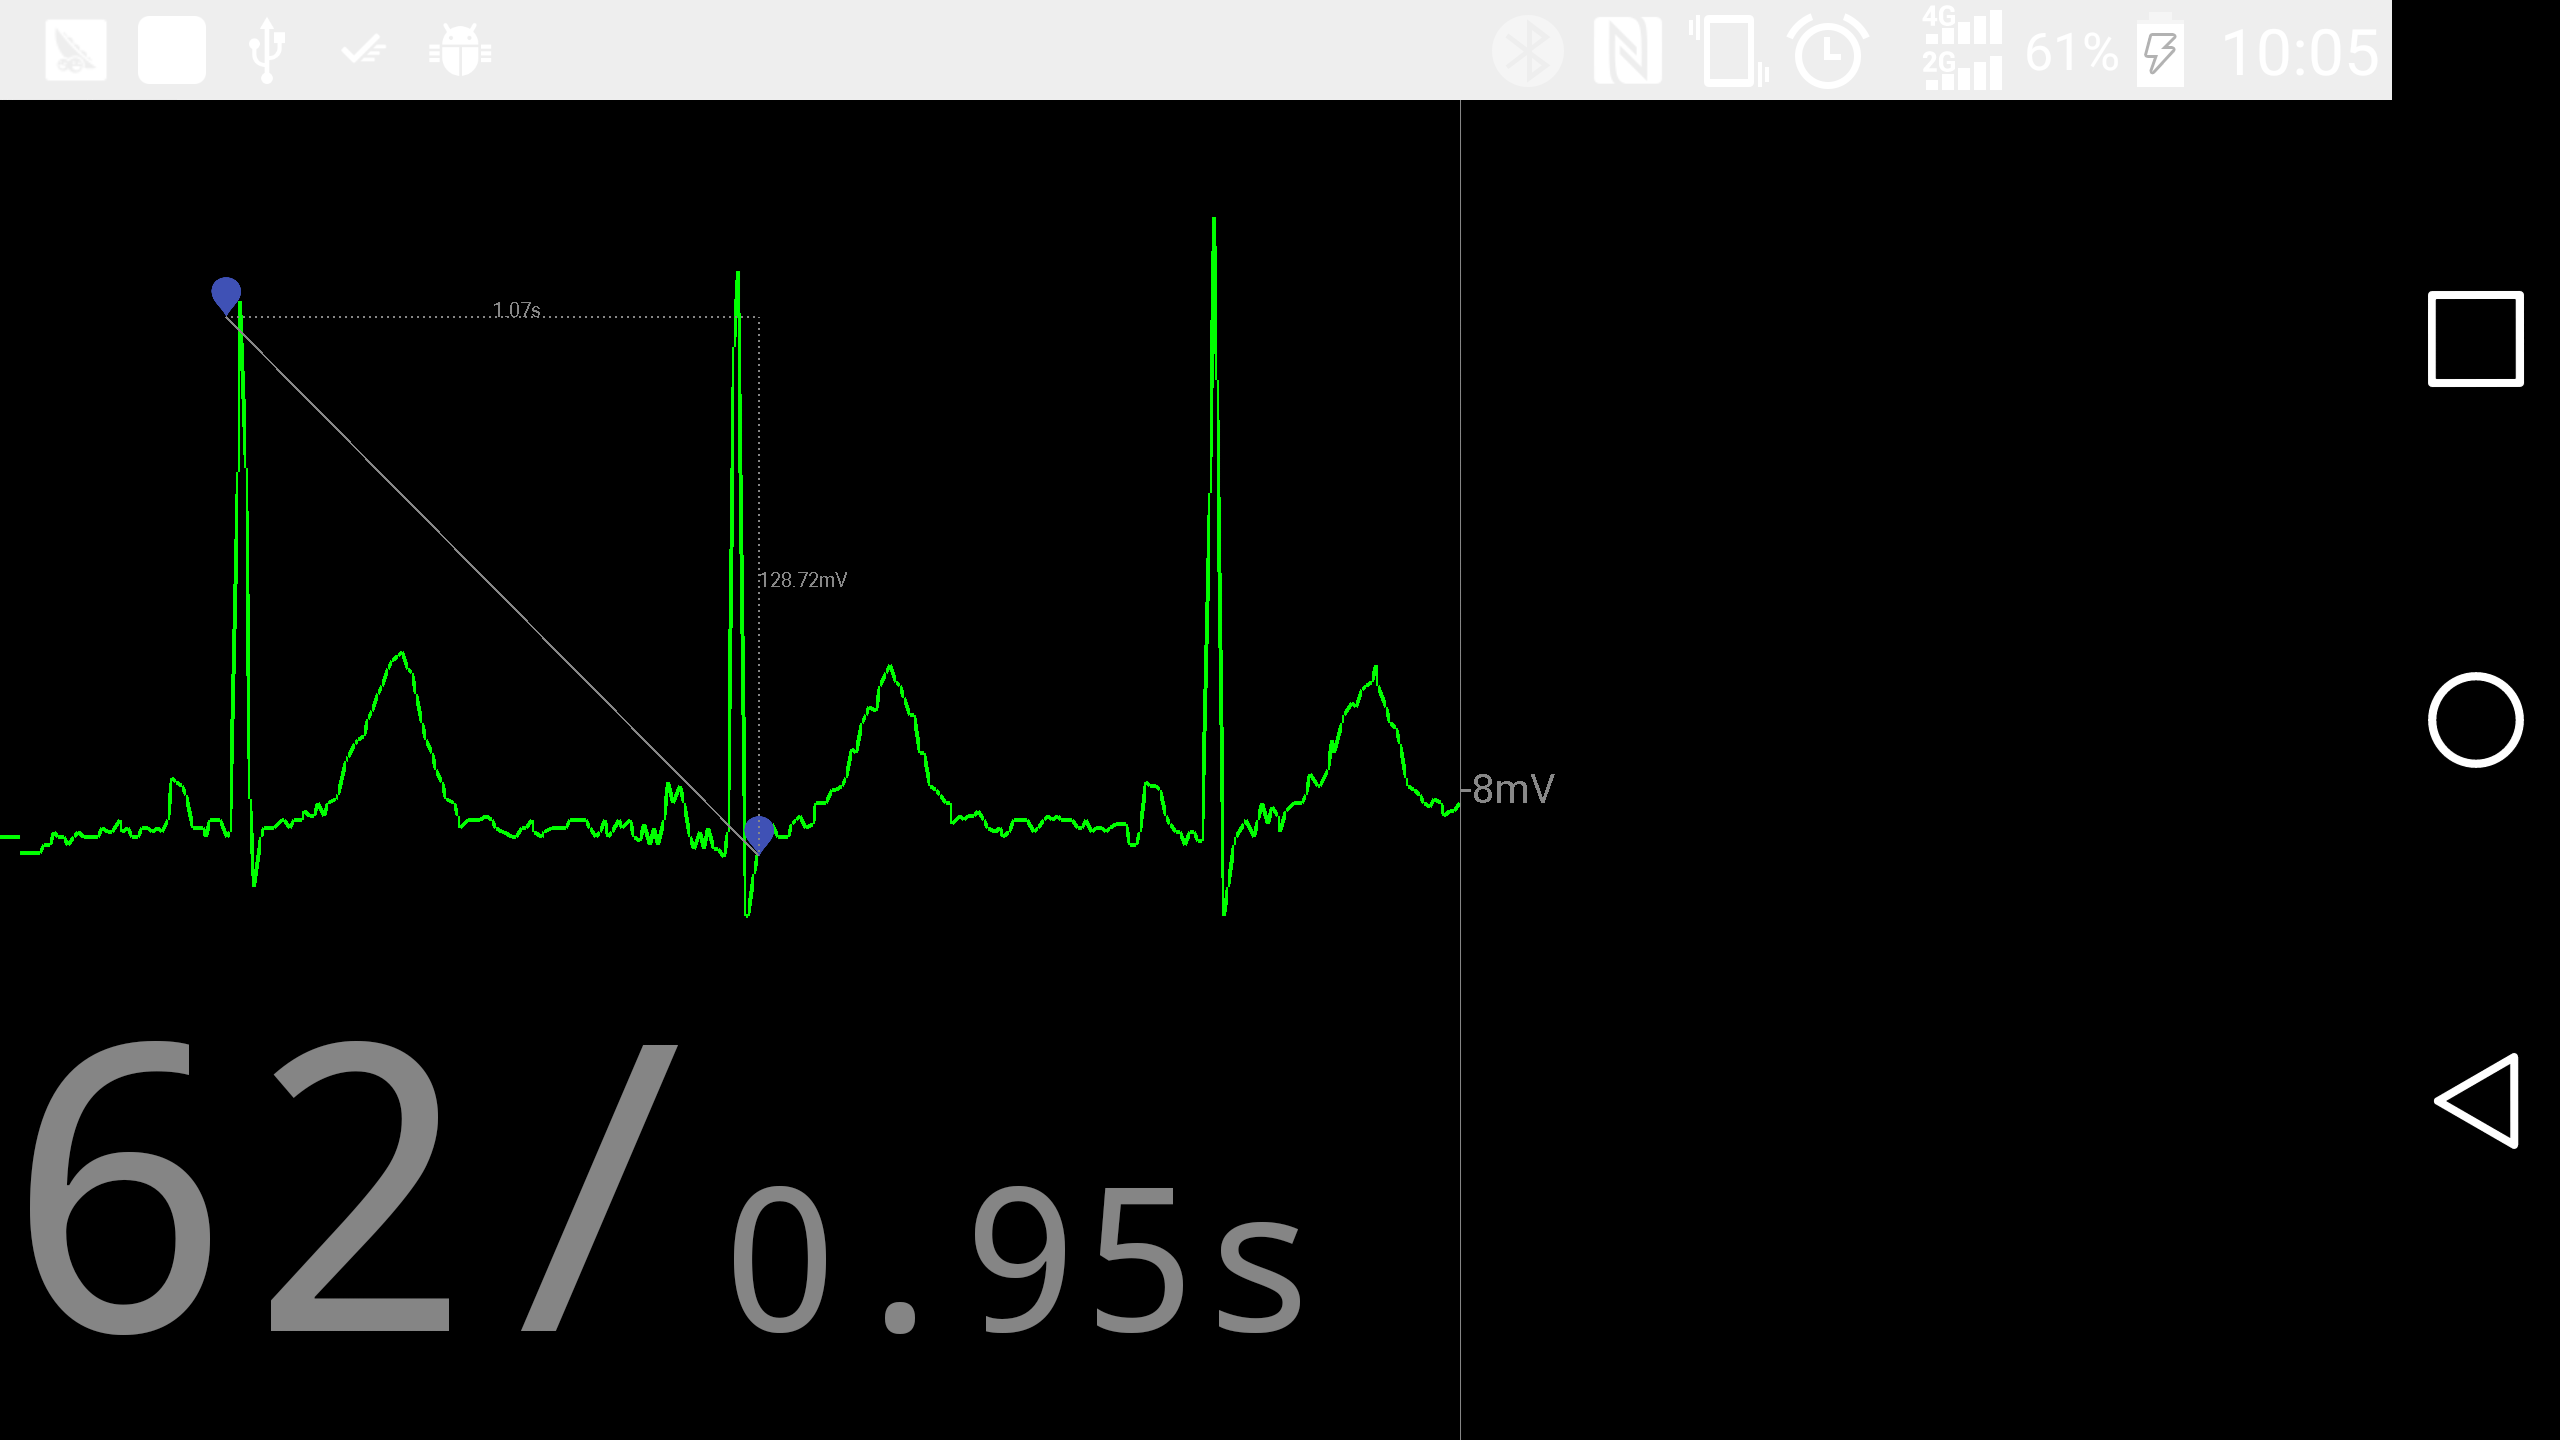
\includegraphics[width=0.6\textwidth]{fig5-1b.png}}
    \caption{探测R峰的过程}
  \label{fig5-1} %% label for entire figure
\end{figure}

\subsection{结论与展望}
本研究是对Android平台有效展示ECG信号的一次尝试。综合来看,本研究所达到的结果有:
\begin{enumerate}
\item 提出了适用于Android平台的ECG波形显示方法,能够更有效地显示波形;
\item 提出了能够与用户交互的波形测量方法,方便波形测量;
\item 提出了一种新的、适用于嵌入式平台的R峰检测算法,并且能够稳定、准确地检测R峰;
\item 实现了基于SQLite的ECG信号数据库,方便管理。
\end{enumerate}

在未来的研究中,基于Android的ECG监测记录应用应向更加实用、更加智能的方向发展。针对不同的用户,应用应能够提供不同的服务来加以适应:如针对医务工作者,应用提供更多的数据以供分析;针对患者,应用提供更加全面的监控或警报功能;针对不同年龄的用户,应用设立不同的监控标准。同时,其采用的信号分析方法也应该具有更高的效率和准确度,以确保在高配置和低配置的设备上均能够流畅运行。最后,相关应用应完成对12个导联的同步支持,这意味着实现更高的蓝牙串口传输速率,或更多的蓝牙设备连接。
